\documentclass[border=10pt]{standalone}

\usepackage{tikz}
\usepackage{tikzsymbols}
\usetikzlibrary{calc,patterns,shapes.geometric}

\def\centerarc[#1](#2)(#3:#4:#5){\draw[#1] ($(#2)+({#5*cos(#3)},{#5*sin(#3)})$) arc (#3:#4:#5);}

\begin{document}
	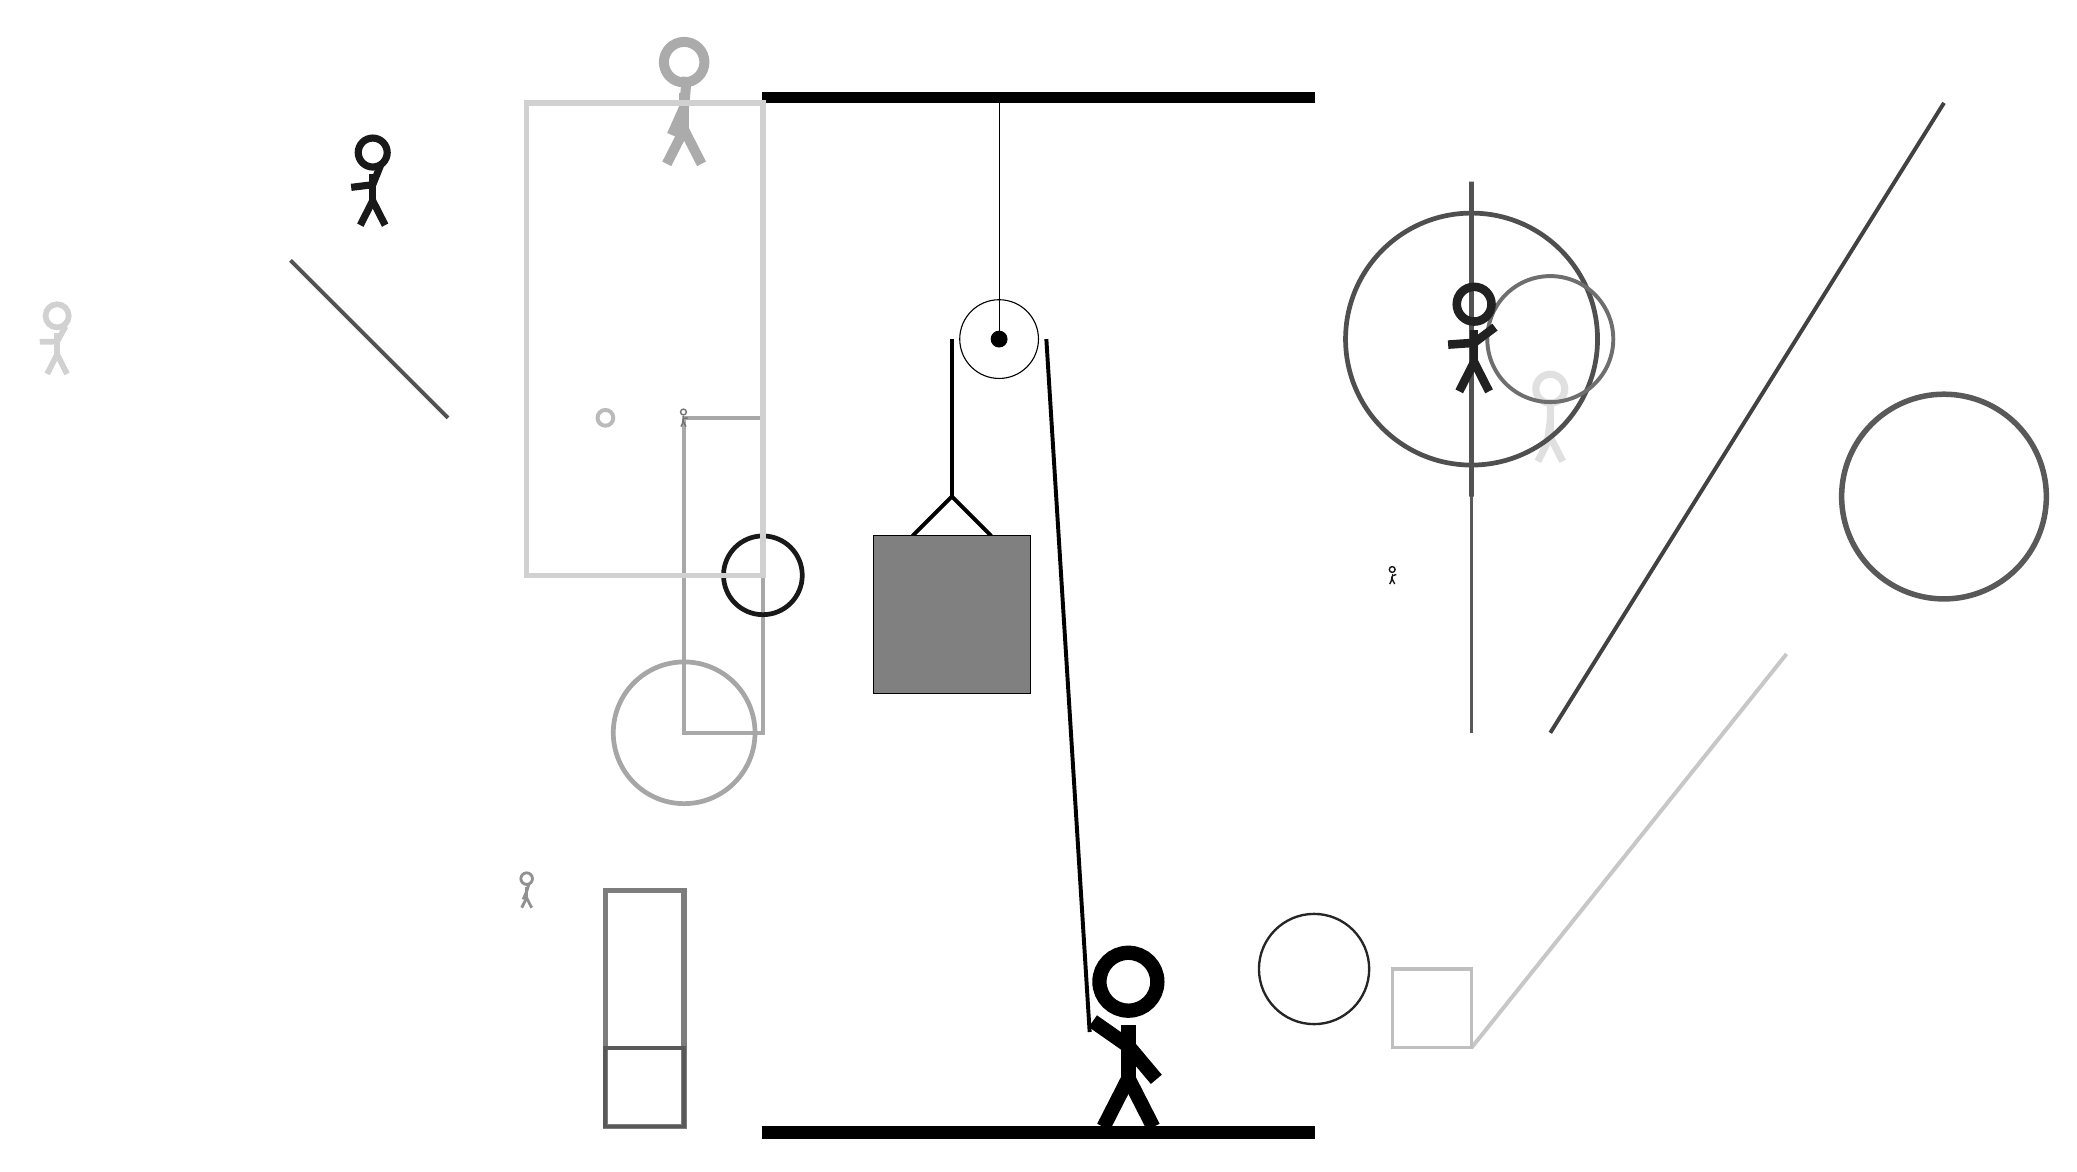
\begin{tikzpicture}
		%%%%% START %%%%%
		
		\draw[fill=black] (-2, 10) rectangle (5, 10.125);
		
		\draw (1, 7) circle (0.5);
		\draw[fill=black] (1, 7) circle (0.1);
		\draw (1, 10) -- (1, 7);
		
		\draw[line width=0.5mm] (-0.1, 4.5) -- (0.4, 5.0) -- (0.9, 4.5);
		\draw[fill=black!50] (-0.6, 4.5) rectangle (1.4, 2.5);
		
		\draw[line width=0.5mm] (0.4, 7) -- (0.4, 5.0);
		\centerarc[line width=0.5mm](1, 7)(0:180:0.6);
		\draw[line width=0.5mm](1.6, 7) -- (2.15, -1.8);
		
		\node[line width=0.2mm, color=black!90] at (-7, 9) {\Strichmaxerl[5][7][68]};
		
		\node[line width=0.5mm, color=black!12] at (8, 6) {\Strichmaxerl[5][82][89]};
		\node[line width=0.7mm, color=black!43] at (-5, 0) {\Strichmaxerl[2][66][73]};
		\draw [line width=0.6mm, color=black!69](7, 7) circle (1.6);
		
		\draw[line width=0.5mm, color=black!22](7, -2) -- (11, 3);
		\draw[line width=0.7mm, color=black!51] (-4, 0) rectangle (-3, -3);
		
		\draw[line width=0.7mm, color=black!32] (-2, 4) rectangle (-5, 10);
		
		\draw [line width=0.7mm, color=black!65](13, 5) circle (1.3);
		\node[line width=0.7mm, color=black!33] at (-3, 10) {\Strichmaxerl[7][66][85]};
		
		\draw[line width=0.3mm, color=black!65] (7, 2) rectangle (7, 8);
		\draw[line width=0.5mm, color=black!34] (-2, 6) rectangle (-3, 2);
		\draw [line width=0.6mm, color=black!90](-2, 4) circle (0.5);
		\draw[line width=0.7mm, color=black!68] (7, 5) rectangle (7, 9);
		
		\draw [line width=0.3mm, color=black!85](5, -1) circle (0.7);
		\node[line width=0.5mm, color=black!55] at (-3, 6) {\Strichmaxerl[1][78][8]};
		\draw[line width=0.7mm, color=black!18] (-2, 10) rectangle (-5, 4);
		\draw [line width=0.5mm, color=black!57](8, 7) circle (0.8);
		\draw[line width=0.5mm, color=black!68](-6, 6) -- (-8, 8);
		\draw[line width=0.5mm, color=black!65] (-4, -3) rectangle (-3, -2);
		\draw[line width=0.5mm, color=black!74](8, 2) -- (13, 10);
		\draw [line width=0.6mm, color=black!35](-3, 2) circle (0.9);
		\node[line width=0.5mm, color=black!90] at (6, 4) {\Strichmaxerl[1][79][20]};
		\node[line width=0.3mm, color=black!18] at (-11, 7) {\Strichmaxerl[4][1][61]};
		\node[line width=0.3mm, color=black!87] at (7, 7) {\Strichmaxerl[6][4][37]};
		\draw[line width=0.4mm, color=black!25] (6, -1) rectangle (7, -2);
		
		\draw [line width=0.5mm, color=black!27](-4, 6) circle (0.1);
		
		\node at (2.6, -1.9) {\Strichmaxerl[10][-35][-50]};
		
		\draw[fill=black] (-2, -3) rectangle (5, -3.15);
		
		%%%%% END %%%%%
	\end{tikzpicture}
\end{document}